\documentclass[conference]{IEEEtran}
% Build:  pdflatex main && bibtex main && pdflatex main && pdflatex main   (or: make -C paper)
\usepackage[T1]{fontenc}
\usepackage{lmodern}
\usepackage{amsmath}
\usepackage{graphicx}
\usepackage{booktabs}
\usepackage{xcolor}
\usepackage{tikz}
\usetikzlibrary{arrows.meta,positioning,fit}
\usepackage{cite}
\usepackage{url}
\usepackage{microtype}
\usepackage[hidelinks]{hyperref}

% Values still to be measured on a real board are shown in red.
\newcommand{\tbd}[1]{\textcolor{red}{#1}}

\begin{document}

\title{Calibrated TinyML for Lone-Worker Safety:\\Fall and Man-Down Detection with an 18\,kB Int8 CNN on the ESP32}

\author{\IEEEauthorblockN{\tbd{Author names}}
\IEEEauthorblockA{\tbd{Department, University}\\
\tbd{City, Country}\\
\tbd{email}}}

\maketitle

\begin{abstract}
A worker who falls or collapses alone needs help to come to them. We present an open,
end-to-end wearable system that detects falls, motionless ``man-down'' collapses and
abnormal vital signs entirely on an ESP32 microcontroller and delivers acknowledged alerts
to a supervisor's web application. Fall detection uses a 7{,}169-parameter
one-dimensional CNN, quantised to int8 (18.6\,kB), on 2.56\,s windows of a waist-worn
inertial sensor evaluated every 0.5\,s. In 5-fold subject-wise cross-validation on all
5{,}057 recordings of the 32 KFall subjects, replayed exactly as the device processes
them, the model detected 2{,}346 of 2{,}346 falls (95\,\% CI 99.84--100\,\%) with 5 false
alarms in 6.3\,h of daily activities (0.79/h) and a median of 0.82\,s from impact to
alarm. A random forest and an impact-plus-posture threshold rule were statistically
indistinguishable on this benchmark (exact McNemar $p \geq 0.38$), so we report what does
separate them: with the sensor mounted 45$^\circ$ away from the training orientation the
augmented CNN still detected 98.7\,\% of falls at 7.1 false alarms/h, against 94.7\,\% and
50.3/h without augmentation and 87.2\,\% for the threshold rule, which also needs
2.3\,s longer to alarm. A two-pose calibration on the device removes most of that
misalignment. The firmware is verified without hardware: its C signal chain reproduces the
Python reference decision-for-decision, the int8 model runs bit-exactly in an ESP32
emulator, and a 250\,s scripted scenario passes end to end, including a supervisor outage.
Code, firmware and web application are released.
\end{abstract}

\begin{IEEEkeywords}
fall detection, man-down, TinyML, edge AI, ESP32, wearable sensors, occupational safety, quantisation
\end{IEEEkeywords}

\section{Introduction}
Falls are a leading cause of injury, and the consequences grow with the time a person lies
without help~\cite{igual2013challenges,mubashir2013survey}. Lone workers---on construction
sites, in warehouses, on night shifts---face the same risk with nobody nearby to raise the
alarm. A wearable alarm for them has four requirements: (i) it must decide on the body, so
that detection does not depend on network coverage; (ii) it must alarm within about a
second, yet let the worker cancel a false alarm; (iii) it must stay quiet during normal
work, or it will be switched off; and (iv) an alert must reliably reach a supervisor, and
the worker must learn that help is coming.

Wearable fall detection has moved from accelerometer thresholds~\cite{bourke2007threshold,kangas2008comparison}
to machine learning and deep networks~\cite{santos2019cnn,musci2021rnn,ramachandran2020survey},
and microcontroller inference has become practical with frameworks such as TensorFlow Lite
Micro~\cite{david2021tflm} and int8 quantisation~\cite{jacob2018quantization}. Two gaps
remain between published detectors and a device a worker can wear. First, most results are
window-level scores on a fixed sensor orientation, whereas a worn device runs a sliding
decision rule on whatever orientation the strap happens to give. Second, detection is only
one link: the device must also handle collapses without an impact, sensor failures,
unreliable vitals during movement and lost network messages.

\textbf{Contributions.} (1) A complete open system---ESP32 firmware, a supervisor web
application and a reproducible training pipeline---for fall, man-down and vital-sign
alerts with acknowledged, store-and-forward delivery. (2) A deployment-faithful evaluation:
every KFall recording is replayed through the device's own decision rule under
subject-wise cross-validation, with false alarms per hour and impact-to-alarm latency, and
exact confidence intervals. (3) Baselines and ablations showing that on KFall the
detectors are statistically tied, while robustness to sensor mounting, latency and memory
footprint separate them. (4) Rotation augmentation combined with a two-pose on-device
calibration, so the sensor can be worn in any orientation. (5) A hardware-free
verification chain that checks the firmware against the reference implementation at
three levels.

\section{Related Work}
Threshold algorithms detect an impact as a peak in acceleration magnitude, often confirmed
by a lying posture~\cite{bourke2007threshold,kangas2008comparison}. They are cheap and
transparent but sensitive to thresholds and orientation. Learning-based methods range from
classical classifiers on hand-crafted features to convolutional and recurrent
networks~\cite{santos2019cnn,musci2021rnn}; surveys
summarise the field and its open problems---realistic falls, false-alarm rates and
usability~\cite{igual2013challenges,mubashir2013survey,ramachandran2020survey}. Public
datasets such as SisFall~\cite{sucerquia2017sisfall} and KFall~\cite{yu2021kfall} made
comparisons possible; Casilari \emph{et al.}~\cite{casilari2017datasets} analyse their
differences. KFall provides a lower-back inertial sensor and labelled impact frames for 32
subjects, which allows latency to be measured. On the embedded side, TensorFlow Lite
Micro~\cite{david2021tflm} and benchmarks such as MLPerf Tiny~\cite{banbury2021mlperftiny}
established microcontroller inference; integer-only quantisation~\cite{jacob2018quantization}
makes such models small and fast. Our focus is the system around the model and an
evaluation that mirrors deployment.

\section{System}

\begin{figure}[t]
\centering
\resizebox{\columnwidth}{!}{%
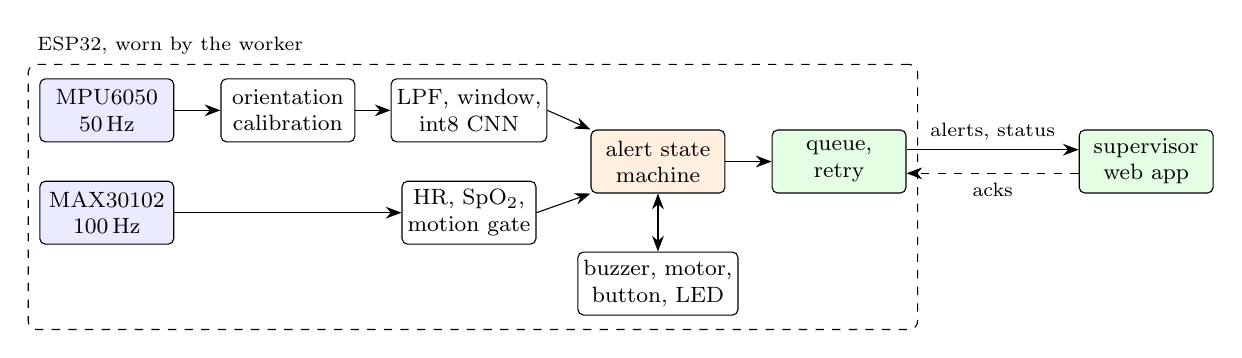
\begin{tikzpicture}[font=\footnotesize, >={Stealth[length=2mm]},
  box/.style={draw, rounded corners=2pt, align=center, minimum height=8mm, minimum width=17mm, inner sep=2pt, fill=#1},
  box/.default=white]
\node[box=blue!8]   (imu) at (0,0)      {MPU6050\\50\,Hz};
\node[box=blue!8]   (ppg) at (0,-1.3)   {MAX30102\\100\,Hz};
\node[box]          (cal) at (2.3,0)    {orientation\\calibration};
\node[box]          (cnn) at (4.6,0)    {LPF, window,\\int8 CNN};
\node[box]          (vit) at (4.6,-1.3) {HR, SpO$_2$,\\motion gate};
\node[box=orange!12] (fsm) at (7.0,-0.65) {alert state\\machine};
\node[box]          (io)  at (7.0,-2.2) {buzzer, motor,\\button, LED};
\node[box=green!10] (net) at (9.3,-0.65) {queue,\\retry};
\node[box=green!10] (web) at (13.2,-0.65) {supervisor\\web app};
\draw[->] (imu) -- (cal);
\draw[->] (cal) -- (cnn);
\draw[->] (ppg) -- (vit);
\draw[->] (cnn.east) -- (fsm.north west);
\draw[->] (vit.east) -- (fsm.south west);
\draw[<->] (fsm) -- (io);
\draw[->] (fsm) -- (net);
\draw[->] ([yshift=1.5mm]net.east) -- node[above, font=\scriptsize]{alerts, status} ([yshift=1.5mm]web.west);
\draw[->, dashed] ([yshift=-1.5mm]web.west) -- node[below, font=\scriptsize]{acks} ([yshift=-1.5mm]net.east);
\node[draw, dashed, rounded corners=3pt, inner xsep=4pt, inner ysep=5pt, fit=(imu)(ppg)(io)(net)(cnn),
      label={[font=\scriptsize, anchor=south west]north west:ESP32, worn by the worker}] {};
\end{tikzpicture}}
\caption{System overview. All detection runs on the worn ESP32; only alerts, status and
acknowledgments use the network.}
\label{fig:system}
\end{figure}

\subsection{Hardware}
The device (Fig.~\ref{fig:system}) is an ESP32 development board with an MPU6050
accelerometer and gyroscope ($\pm$16\,g, $\pm$2000\,$^\circ$/s, 50\,Hz FIFO) worn at the
lower back, a MAX30102 pulse oximeter on a fingertip, an active buzzer, a coin vibration
motor and one button; the parts cost about USD 15--25. The same firmware builds for the
ESP32-S3.

\subsection{Signal chain and fall detector}
Each inertial sample is rotated into the frame of the training data (Section~\ref{sec:cal}),
low-pass filtered (causal 4th-order Butterworth, 5\,Hz) and appended to a 128-sample
(2.56\,s) window. Every 25 samples (0.5\,s) the window is standardised, quantised and
classified by the int8 CNN; a fall is suspected when two consecutive windows exceed the
threshold. The filter state is initialised from the first sample, so the C implementation
matches the Python reference exactly.

\subsection{Alert state machine}
A suspected fall starts a pre-alarm (buzzer and vibration). Pressing ``I'm OK'' within
10\,s cancels it; otherwise an \texttt{ALERT\_FALL} is sent after 5\,s of stillness (motion
below 0.05\,g) or when the 10\,s run out, with posture and impact force. \emph{Man-down}
catches collapses without an impact: lying (tilt above 60$^\circ$) and motionless for
30\,s, or upright and motionless for 180\,s, starts a 15\,s pre-alarm that movement or the
button cancels. Vital-sign alarms (heart rate outside 45--140\,bpm or SpO$_2$ below
90\,\% for 10\,s) are \emph{motion-gated}: they are suspended while the mean motion over
10\,s exceeds 0.35\,g, because photoplethysmography is unreliable during exertion. A
skin-contact check suspends vitals and man-down while the device is not worn, and a
sensor-fault monitor reports a frozen or silent motion sensor (\texttt{DEVICE\_FAULT}).

\subsection{Reliable alerting and supervisor application}
Alerts carry an identifier \texttt{boot-n} and wait in a queue that is retried with
exponential back-off (up to 30\,s) until the supervisor confirms receipt, so a network
outage delays but never loses them. The supervisor web application (Python standard
library, SQLite, Server-Sent Events; Fig.~\ref{fig:dashboard}) shows workers, vitals and
alerts live, sounds an alarm, and lists acknowledged identifiers in every reply; on receipt
the device switches to a ``help is on the way'' signal. Devices report status every 5\,s.

\begin{figure}[t]
\centering
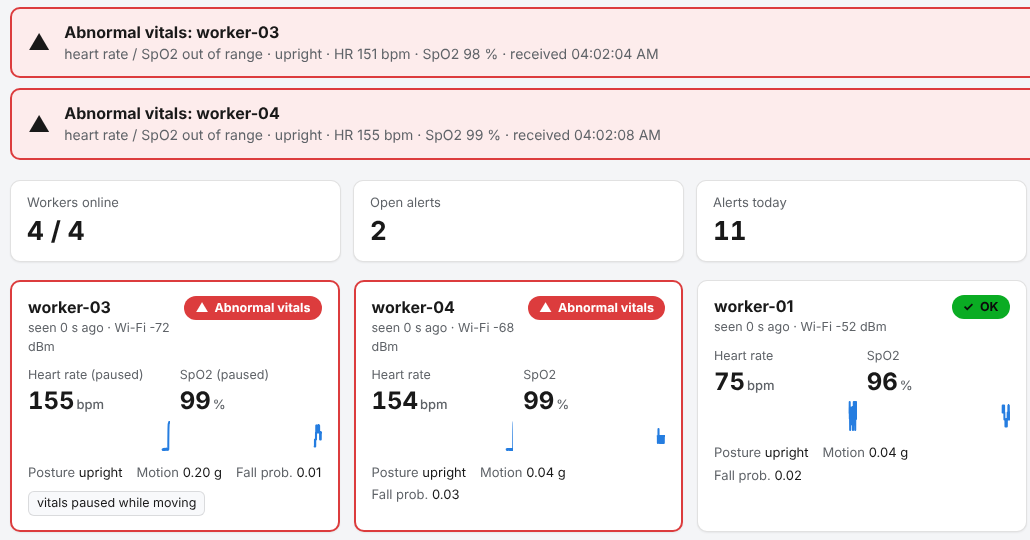
\includegraphics[width=\columnwidth]{figs/dashboard.png}
\caption{Supervisor web application with simulated workers: open alerts with elapsed
time and an acknowledge button, and per-worker vitals.}
\label{fig:dashboard}
\end{figure}

\subsection{Setup and orientation calibration}\label{sec:cal}
A prebuilt image is flashed from the browser. On first start the device opens a Wi-Fi
access point with a captive setup page for the network, supervisor address and worker
name. The same page calibrates the orientation in two still poses. Standing upright gives
the unit gravity reading $\mathbf{a}$ in the sensor frame; bending forward by about
45$^\circ$ gives $\mathbf{b}$. The body's forward axis is
$\mathbf{f} = -(\mathbf{b} - (\mathbf{b}\!\cdot\!\mathbf{a})\mathbf{a}) / \lVert\cdot\rVert$,
and the rotation into the KFall frame ($+y$ down, $+z$ forward) has rows
$\mathbf{y}\times\mathbf{f}$, $\mathbf{y} = -\mathbf{a}$ and $\mathbf{f}$. Calibration is
rejected if the device moves ($\sigma_{|a|} > 0.05$\,g) or the bend is below 20$^\circ$.

\begin{table*}[t]
\centering
\caption{Subject-wise 5-fold cross-validation on all 5{,}057 KFall recordings, device decision rule.
Brackets: exact 95\,\% confidence intervals. Latency: time from the labelled impact to the alarm.}
\label{tab:main}
\footnotesize
\setlength{\tabcolsep}{4pt}
\begin{tabular}{lcccccl}
\toprule
Method & Falls & Sensitivity (\%) & Specificity (\%) & False alarms/h & Latency (s) & Size \\
 & detected & & (recordings) & of activity & median / p95 & \\
\midrule
1D-CNN (deployed) & 2346/2346 & 100 [99.84, 100] & 99.82 [99.57, 99.94] & 0.79 [0.26, 1.85] & 0.82 / 1.10 & 7.2k params, int8 18.6\,kB \\
\quad no augmentation & 2344/2346 & 99.91 [99.69, 99.99] & 99.85 [99.62, 99.96] & 0.64 [0.17, 1.63] & 0.82 / 1.10 & same \\
\quad accelerometer only & 2346/2346 & 100 [99.84, 100] & 99.85 [99.62, 99.96] & 0.64 [0.17, 1.63] & 0.84 / 1.11 & 6.8k params \\
\quad 1.28\,s window & 2343/2346 & 99.87 [99.63, 99.97] & 99.78 [99.52, 99.92] & 0.95 [0.35, 2.07] & 0.78 / 1.06 & 175k MAC \\
\quad 3.84\,s window & 2346/2346 & 100 [99.84, 100] & 99.78 [99.52, 99.92] & 0.95 [0.35, 2.07] & 0.92 / 1.86 & 523k MAC \\
Random forest & 2342/2346 & 99.83 [99.56, 99.95] & 100 [99.86, 100] & 0.00 [0, 0.59] & 0.86 / 1.14 & 40k--49k tree nodes \\
Impact + posture rule & 2345/2346 & 99.96 [99.76, 100] & 99.78 [99.52, 99.92] & 0.95 [0.35, 2.07] & 3.08 / 3.12 & 2 thresholds \\
\bottomrule
\end{tabular}
\end{table*}

\section{Fall Detection Model}
\textbf{Data.} KFall~\cite{yu2021kfall}: 32 young adults, 21 activities of daily living
(ADL) and 15 fall types, lower-back sensor at 100\,Hz with labelled impact frames; 5{,}057
usable recordings (2{,}346 falls, 2{,}711 ADL, 6.3\,h of ADL). We keep the six channels
an MPU6050 provides and resample to 50\,Hz.

\textbf{Windows.} Training fall windows are cut with the labelled impact at nine
positions between 35\,\% and 85\,\% of the window; ADL windows every 32 samples.

\textbf{Network.} Three Conv1D blocks (16, 32, 32 filters; kernels 7, 5, 3) with batch
normalisation, ReLU and max-pooling, global average pooling, dropout 0.3, a 16-unit dense
layer and a sigmoid output: 7{,}169 parameters and 349k multiply--accumulates per window,
using only operators supported by TensorFlow Lite Micro.

\textbf{Training.} Adam (learning rate $10^{-3}$, halved on plateau), batch 256, class
weights, up to 40 epochs with early stopping on validation loss (validation AUC saturates
at 1.0 after one epoch and is useless as a stopping signal). Each batch is augmented with a
random rotation (rotation vector $\sim\mathcal{N}(0, 10^\circ)$ per axis), per-channel gain
0.92--1.08 and sensor noise.

\textbf{Threshold.} On the validation subjects many thresholds tie at the maximum F1;
we take the middle of the longest tied run rather than its lowest value, which is the most
alarm-prone choice.

\textbf{Quantisation.} Full-integer post-training quantisation with 1{,}000
representative windows gives an 18.6\,kB model; on the test subjects its decisions are
identical to the float model's.

\section{Evaluation Method}
We use 5-fold cross-validation grouped by subject; inside each fold, one eighth of the
training subjects (at least two) form the validation set. Every recording is therefore
tested exactly once by a model that never saw its subject. Recordings are streamed through
the device rule (window every 0.5\,s, two consecutive positives). A fall counts as detected
if an alarm occurs from 1\,s before the labelled impact onwards; latency is the alarm time
minus the impact time. Every alarm during an ADL recording is a false alarm; we report
false alarms per hour of ADL with Poisson intervals and per-recording specificity with
Clopper--Pearson intervals. Methods are compared with exact McNemar tests on paired
recording-level outcomes.

\textbf{Baselines.} A random forest (300 trees) on 38 window features (per-channel mean,
standard deviation, minimum, maximum and range; magnitude statistics; tilt at the start
and end of the window), trained on the same windows with the same augmentation and using
the same decision rule. An impact-plus-posture rule after~\cite{bourke2007threshold}:
acceleration magnitude above an upper threshold, followed 2--3\,s later by a tilt above a
posture threshold, both tuned per fold on the training subjects (selected: 1.8\,g and
60$^\circ$ in four folds, 45$^\circ$ in one). \textbf{Ablations:} no augmentation,
accelerometer only, and 1.28\,s or 3.84\,s windows. \textbf{Mounting robustness:} every
test recording is rotated by a fixed angle about a random axis (the same axis for all
methods) and evaluated without retraining.

\section{Results}


\textbf{Detection on KFall.} Table~\ref{tab:main} shows that the deployed CNN detected
every fall of every held-out subject, with 5 false alarms in 6.3\,h of ADL and an alarm a
median 0.82\,s after impact (85\,\% within 1\,s; no fall recording raised an alarm
more than 1\,s before its impact). All methods lie within a fraction of a percent of each other, and no difference
to the CNN is significant (McNemar $p$ between 0.38 and 1; e.g.\ random forest: 4
recordings only the CNN got right, 5 only the forest). KFall is effectively saturated at
this level, which is why we report the deployment-relevant properties below. Requiring
one, two or three consecutive positive windows trades 0.95, 0.79 and 0.64 false alarms/h
against median latencies of 0.32, 0.82 and 1.32\,s; three windows missed 4 falls.

\textbf{Sensor mounting.} Fig.~\ref{fig:robust} reports performance when the sensor is
mounted rotated. Up to 30$^\circ$ the augmented CNN keeps 99.9\,\% sensitivity and at most
1.1 false alarms/h. At 45$^\circ$ it detects 98.7\,\% of falls with 7.1 false alarms/h,
whereas the same network without augmentation falls to 94.7\,\% and 50.3/h, the random
forest (whose features include absolute tilt) to 98.1\,\% and 20.0/h, and the threshold
rule to 87.2\,\% and 11.0/h. At 0$^\circ$ augmentation makes no significant difference (McNemar $p = 1$); beyond
20$^\circ$ it is decisive; the on-device calibration of Section~\ref{sec:cal} keeps a worn device
near the left end of these curves.

\begin{figure}[t]
\centering
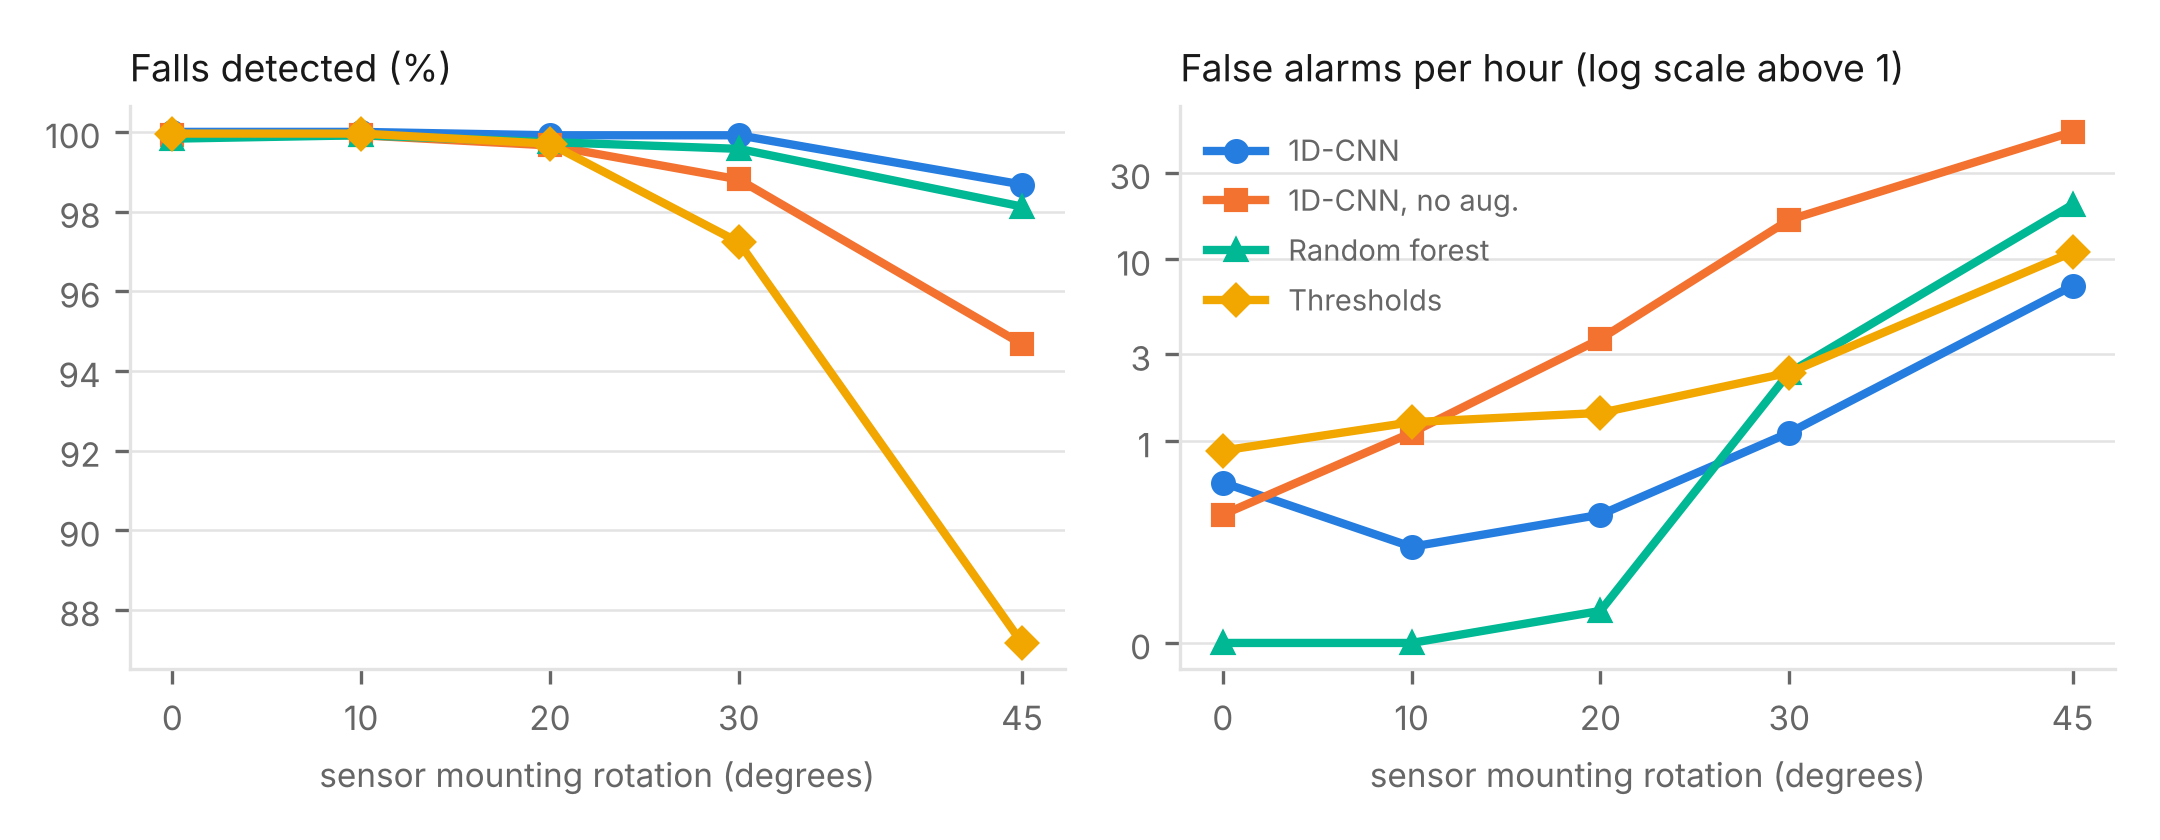
\includegraphics[width=\columnwidth]{figs/fig_robustness.png}
\caption{Falls detected and false alarms per hour when every test recording is rotated by a
fixed angle about a random axis (no retraining).}
\label{fig:robust}
\end{figure}

\begin{figure}[t]
\centering
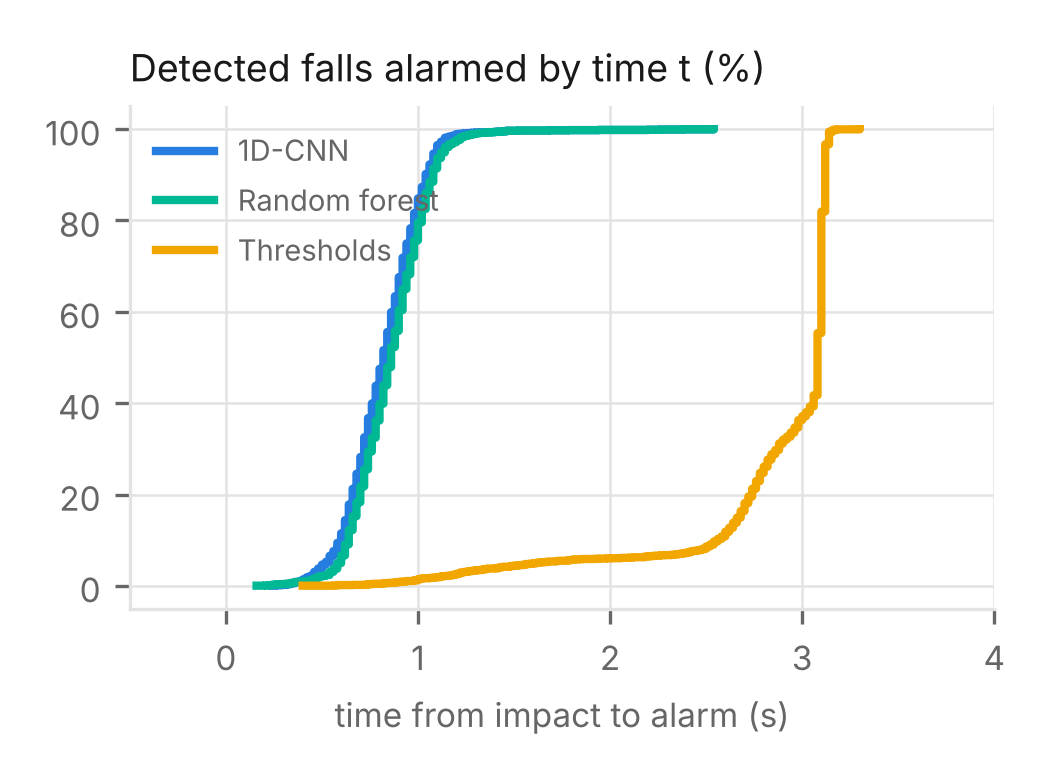
\includegraphics[width=0.8\columnwidth]{figs/fig_latency.png}
\caption{Cumulative distribution of the time from impact to alarm for detected falls.}
\label{fig:latency}
\end{figure}

\textbf{Latency.} The threshold rule must wait for the posture after the impact and alarms
after 3.1\,s; the learned detectors alarm after 0.8--0.9\,s (Fig.~\ref{fig:latency}). In
the full system the pre-alarm begins at that moment, and the supervisor is notified after
the worker's 10\,s cancel window or 5\,s of stillness.

\textbf{Footprint.} The int8 CNN needs 18.6\,kB of flash and a 16\,kB tensor arena of
which 7.3\,kB are used (ESP32). The random forest needs about 40k--49k tree nodes per fold,
roughly 0.4--0.5\,MB at 10 bytes per node, for no measurable gain on KFall and less
robustness. The accelerometer-only variant performs like the six-channel model, which
would allow the gyroscope to be switched off to save power. The complete firmware image
(Wi-Fi, setup web server, HTTP client, model) is 1.06\,MB, 68\,\% of the 1.5\,MB
application partition, with 127\,kB of static RAM in use (ESP-IDF 5.5), and one inference
takes \tbd{[measured on the board]}\,ms at 240\,MHz, printed by the firmware at boot, well
inside the 500\,ms decision period.

\section{Verification Without Hardware}
Three automated levels check that the firmware behaves like the evaluated model.
(1)~\emph{Parity:} the portable C core (filter, windows, quantisation, decision rule,
vital-sign estimators, state machine) is compiled on a PC and compared with the Python
reference; on the 957 recordings of the six original test subjects it reproduces every
decision. (2)~\emph{Bit-exact inference:} the int8 model runs inside an emulated ESP32
(QEMU) on 28 reference windows; all outputs equal those of the TensorFlow Lite reference
kernels. (3)~\emph{End to end:} the full firmware replays a scripted 250\,s scenario
(normal work, jogging with motion artefacts in the pulse signal, a fall, a cancelled fall,
tachycardia, a slow collapse, a cancelled man-down, standing still and a frozen sensor) in
the emulator, with the supervisor started 20\,s late; all 11 expected events occur at the
expected times, and the queued alerts arrive in order and are acknowledged. These checks,
plus 17 web-application tests, run on every commit.

\section{Discussion and Limitations}
KFall contains simulated falls by young adults on mats, and its ADL clips are short and
dense with difficult movements; false alarms per hour measured on them are therefore
pessimistic for a working shift, and sensitivity to real occupational falls is unknown.
Because all detectors saturate on KFall, cross-dataset evaluation (for example on
SisFall~\cite{sucerquia2017sisfall}, which the pipeline supports) and recordings from the
device itself are the most important next steps. The vital-sign estimators were checked on
synthetic signals only and are not clinically validated. The orientation calibration
assumes a still upright stance and a clean forward bend; residual errors of a few degrees
are covered by augmentation, as Fig.~\ref{fig:robust} shows. Finally, inference time and
battery life must be measured on boards, and the system has not yet been worn in a field
trial. A demonstration feature replays a recorded synthetic fall into the sensor stream so
that the full alert chain can be shown safely; it must be disabled in deployed devices.

\section{Conclusion}
A 7k-parameter int8 CNN on an ESP32 detects all KFall falls of unseen subjects with under
one false alarm per hour of dense activity and alarms within a second of impact. Its
advantage over a random forest and a threshold rule is not accuracy on KFall, where they
are tied, but robustness to how the device is worn, alarm latency and footprint. Combined
with on-device calibration, man-down and motion-gated vitals, acknowledged store-and-forward
alerting and an automated verification chain, it forms a complete, reproducible baseline
for lone-worker safety that others can build, test and extend.

\section*{Data and Code Availability}
Training pipeline, experiment scripts, firmware, web application and hardware
instructions are available at \tbd{[repository URL]}. KFall is available from its authors
on request~\cite{yu2021kfall}; no KFall data is redistributed with the code.

\section*{Acknowledgment}
We thank the authors of KFall for making their dataset available. \tbd{Funding and other
acknowledgments.}

\bibliographystyle{IEEEtran}
\bibliography{refs}

\end{document}
